%\documentclass[aps,prd,nofootinbib,amsmath,notitlepage]{revtex4-1}
\documentclass[11pt]{article}
\usepackage{jcappub}
\usepackage{amssymb,esvect,amsmath,graphicx,latexsym,amsthm,slashed,eso-pic,fullpage}  
\usepackage[final]{pdfpages}
\DeclareMathOperator{\ev}{eV} \DeclareMathOperator{\kev}{KeV} \DeclareMathOperator{\mev}{MeV} \DeclareMathOperator{\gev}{GeV} \DeclareMathOperator{\tev}{TeV} \DeclareMathOperator{\cm}{cm} \DeclareMathOperator{\barn}{barn} \DeclareMathOperator{\g}{g} \DeclareMathOperator{\km}{km} \DeclareMathOperator{\pb}{pb} \DeclareMathOperator{\s}{s} \DeclareMathOperator{\yr}{yr}\DeclareMathOperator{\gyr}{Gyr} \DeclareMathOperator{\kg}{kg} \DeclareMathOperator{\mpc}{Mpc} \DeclareMathOperator{\few}{few} \DeclareMathOperator{\kel}{K}
\newcommand{\cA}{{\cal A}} \newcommand{\cC}{{\cal C}} \newcommand{\cD}{{\cal D}} \newcommand{\cE}{{\cal E}} \newcommand{\cF}{{ \cal F}} \newcommand{\cH}{{\cal H}} \newcommand{\cJ}{{\cal J}} \newcommand{\cL}{{\cal L}} \newcommand{\cM}{{\cal M}} \newcommand{\cN}{{\cal N}} \newcommand{\cO}{{\cal O}} \newcommand{\cP}{{ \cal P}} \newcommand{\tp}{{ \tilde p}} \newcommand{\cR}{{\cal R}} \newcommand{\cS}{{\cal S}}
\newcommand{\ep}{\epsilon} \newcommand{\vp}{\varphi} \newcommand{\half}{\frac12}
\newcommand{\ie}{{\it i.e.~}}  \newcommand{\eg}{{\it e.g.~}}
\newcommand{\pt}{\partial} \def\d{{\rm d}}  \def\oL{\overline} \def\wh{\widehat}
\newcommand{\pL}{\left(} \newcommand{\pR}{\right)} \newcommand{\bL}{\left[} \newcommand{\bR}{\right]} \newcommand{\cbL}{\left\{} \newcommand{\cbR}{\right\}} \newcommand{\mL}{\left|} \newcommand{\mR}{\right|}
\newcommand{\beq}{\begin{equation}} \newcommand{\eeq}{\end{equation}}
\newcommand{\bea}{\begin{eqnarray}} \newcommand{\eea}{\end{eqnarray}}
\newcommand{\alg}[1]{\begin{align} \begin{split} #1 \end{split}  \end{align}}
\newcommand{\vev}[1]{\langle {#1} \rangle}
\newcommand{\tenx}[1]{\times 10^{#1}}
\newcommand{\Eq}[1]{Eq.~(\ref{#1})} \newcommand{\Eqs}[2]{Eqs.~(\ref{#1}) and (\ref{#2})} \newcommand{\Eqm}[2]{Eqs.~(\ref{#1}) through (\ref{#2})}
\newcommand{\Sec}[1]{Sec.~\ref{#1}} \newcommand{\Secs}[2]{Secs.~\ref{#1} and \ref{#2}} \newcommand{\Secm}[2]{Secs.~\ref{#1} through \ref{#2}}
\newcommand{\Fig}[1]{Fig.~\ref{#1}} \newcommand{\Figs}[2]{Figs.~\ref{#1} and \ref{#2}}
\newcommand{\Tab}[1]{Tab.~\ref{#1}}
\newcommand{\App}[1]{App.~\ref{#1}}
\DeclareMathOperator{\br}{Br} \DeclareMathOperator{\tr}{Tr}
\newcommand{\arxiv}[1]{{\href{http://arxiv.org/abs/#1}{\tt #1}}}

\newcommand{\sam}[1]{\textcolor{blue}{\textbf{(#1 -- Sam)}}}


\begin{document}
\title{Model Selection with a Single Target:\\Leveraging Annual Modulation to Differentiate Direct Detection Signals}
\author{Samuel Witte,}
\author{Vera Gluscevic, and}
\author{Samuel D. McDermott}


\abstract{
\sam{I've listed the authors as if this is an astro-ph paper, but perhaps it will be more suitable for hep-ph, and should be alphabetical? No need to decide immediately.} Abstract goes here, and it will say lots of interesting stuff when we finally figure out our conclusions, but for now this is just a placeholder. Abstract goes here, and it will say lots of interesting stuff when we finally figure out our conclusions, but for now this is just a placeholder. Abstract goes here, and it will say lots of interesting stuff when we finally figure out our conclusions, but for now this is just a placeholder. Abstract goes here, and it will say lots of interesting stuff when we finally figure out our conclusions, but for now this is just a placeholder.
}

\maketitle

\section{Introduction} \setcounter{page}{2}

Experimental evidence from a vast array of independent sources conclusively demonstrates the existence of a non-baryonic form of matter in the universe. This so-called dark matter is the dominant source of the gravitational potential wells that have determined the large scale structure of the universe, but dark matter particles have yet to be observed in a laboratory setting. Despite an experimental direct detection program that has now been mature for several decades, all evidence in favor of the existence of dark matter is instead furnished by indirect observations of cosmological and astrophysical settings.

There are good reasons to be optimistic that direct detection may be on the cusp of important discoveries, however. As next-generation experiments that incorporate increasingly precise detection technologies come online, we will be pushing through the final parameter space before encountering the astrophysical neutrino background. Luckily, many interesting theories of dark matter predict scattering cross sections in this range. For example, heavy $SU(2)$-doublet and -triplet fermions, such as the Higgsinos and the wino of supersymmetry, are expected to have cross sections of order $\sigma_{\rm SI} \sim \cO(\few\tenx{-48})\cm^2$, fixed by their Standard Model gauge quantum numbers alone \cite{Hill:2011be,Hill:2013hoa,Hill:2014yxa}, while a heavy $SU(2)$-singlet fermion, like the bino, is around an order of magnitude lower depending on its coannihilation partner \cite{Berlin:2015njh}. Models with kinematically suppressed tree-level scattering may also be embedded in more complete dark sectors that have loop-level cross sections in this same range \cite{Ipek:2014gua,McDermott:2014rqa,Appelquist:2015yfa,Appelquist:2015zfa}.

Because so many theories can be accommodated in the parameter space that we will imminently probe, we must plan for the science opportunities associated with the first detection of dark matter particles. The ``inverse problem'' that we will confront upon successful detection of dark matter particles is that of understanding the (high-energy) dark sector dynamics solely by examining (low-energy) recoils of detector elements. In collider physics terms, the luminosity is fixed by the dark matter astrophysics, making measurements of dark matter properties possible only at a single energy scale. We will need to reconstruct the interesting physics of the dark sector at all scales from nuclear recoils alone, despite the fact that the details of the dynamics that link the dark sector to the Standard Model are most likely integrated out at the low energies probed in direct detection experiments.

At the low energies of direct detection experiments, the nuclear responses can be described by an easily exhaustible list of interactions, which have been compactly written down as a nonrelativistic effective field theory \cite{Fitzpatrick:2012ix,Anand:2013yka}. This effective field theory of dark matter direct detection reproduces the nontrivial physics induced by some of the best-motivated UV-complete theories of dark matter \cite{Gresham:2014vja,Gluscevic:2015sqa}. We can look for clues to the nature of the dark sector in several important ways using this effective theory.

At first order, the most important information about the dark sector is contained in the energy spectrum of the scattering. A close examination of the energy spectrum of dark matter scattering in experiments with different nuclei can provide sufficient information to break degeneracies in the dark matter model space as long as the target nuclei have sufficiently complementary nuclear physics characteristics \cite{McDermott:2011hx,Peter:2013aha,Gluscevic:2014vga,Catena:2014epa,Catena:2014hla,Dent:2015zpa,Gluscevic:2015sqa}. Model selection with complementary nuclei is therefore capable of reconstructing the dark matter physics using spectral information alone.

In this work, we will be interested in a different signature of the low-energy physics that can potentially reveal the dynamics of the dark sector. All events at direct detection experiments will be characterized by an energy as well as by a particular time; in collider physics terms, the luminosity has a well-understood time variation. Here, we will investigate how this time-dependence of the direct detection rate can be leveraged to help improve model selection prospects. The annual modulation of the direct detection rate (and its higher harmonics) has been well understood for almost as long as direct detection has been pursued \cite{Freese:1987wu,Freese:2012xd,Lee:2013xxa,Lee:2013wza,DelNobile:2015tza,DelNobile:2015nua,DelNobile:2015rmp}. Here we will demonstrate that, for certain classes of interactions, the additional discrimination power from timing information will allow some of the most popular detector designs to achieve comprehensive model selection \sam{in the G2 experiments? G3? before the neutrino floor? never? just shooting from the hip here. We will say more as we actually get conclusions}. In this way, it may be possible to discriminate between certain models of the dark matter using a single detector element on its own.

The rest of the paper is laid out like \sam{every other good paper you've read, and totally unlike all the bad papers that you usually read}.

\section{Dark Matter Direct Detection in the Lab}


The nuclear recoil energy spectrum is the number count of nuclear recoil events observed per recoil energy $E_R$, per unit time, per unit target mass,
\begin{equation}
\frac{dR}{dE_R dt}(E_R,t) =  \frac{\rho_\chi}{m_T m_\chi} \int\limits_{v_{\mathrm{min}}}^{v_{\mathrm{esc, lab}}}  v f(\mathrm{\mbox{\bf{v}}}|t) \frac{d\sigma_T}{dE_R} (E_R,v) d^3v ,
\label{eq:dRdEr_general}
\end{equation}
where:
\begin{itemize}
\item $\rho_\chi$ and $m_\chi$ are the local dark matter density and the dark matter particle mass
\item $v_\mathrm{min} = \sqrt{m_T E_R/2\mu_T^2}$ is the minimum velocity a dark matter particle of mass $m_\chi$ needs to produce a nuclear recoil of energy $E_R$, where $\mu_T=\frac{m_Tm_\chi}{m_T+m_\chi}$ is the reduced mass of the dark matter particle and the target nucleus
\item $v_{\mathrm{esc, lab}}$ is the escape velocity from the Galactic halo in the lab frame
\item $v$ is the velocity of the dark matter in the lab frame
\item $f(\mathrm{\mbox{\bf{v}}}|t)$ is the observed dark matter velocity distribution, which is generically time-dependent
\item and $d\sigma_T/dE_R=m_T \sigma_T /2\mu_T^2 v^2$ is the differential cross section for dark matter scattering off a nucleus.
\end{itemize}
The differential rate in \Eq{eq:dRdEr_general} is determined by the experimental set up, the dark matter astrophysics, the particle properties of dark matter, the nuclear properties of the target material $T$ (throughout this paper we use $T$ to denote the nuclear target and we reserve $N$ to denote a nucleon, either $n$ or $p$), and the type of interaction between the dark matter and the target. For the purposes of this study, we set the astrophysical parameters to the following values \cite{Bovy:2013raa}: $\rho_\chi=0.3$ GeV/cm$^3$; $v_{\mathrm{esc}} = 544$ km/sec in the Galactic frame; we assume that $f(\mathrm{\mbox{\bf{v}}})$ is a Maxwellian distribution in the Galactic frame, with an rms speed of $155$ km/sec, and a mean speed equal to the Sun's rotational velocity around the Galactic center, $v_\textrm{lag}=220$ km/sec. The underlying particle physics model determines the calculation of the recoil rate through the differential scattering cross section ${d\sigma_T}/{dE_R}$, as discussed in \cite{Gluscevic:2015sqa,Gresham:2014vja}: this has a free normalization with units of cm${}^2$ as well as a discrete set of functional dependences on $E_R$ and $v$, as described in more detail below.

What we describe below as the total rate $R$ of events is the integral of the differential rate within the nuclear-recoil energy range $\cE$ of a given experiment\footnote{For simplicity, in this work we assume unit efficiency of detection, at all energies within the analysis window, for each experiment considered here, and rescale the exposures to take this assumption into account when choosing experimental parameters to represent the capabilities of G2 experiments.}, $R(t)=\int_\cE \frac{dR}{dE_R dt} dE_R$. The total expected number of events $N$ for a target of total mass $\cM$ from a time $t_1$ to $t_2$ over an energy is 
\beq
N =  \cM \int\limits_{t_1}^{t_2} \int\limits_\cE  \frac{dR}{dE_R dt}(E_R,t)\,dE_R \,dt.
\eeq
The total number of events and the differential rate for a given energy and time will be used to define a likelihood function, as described in \cite{Gluscevic:2015sqa}.

\subsection{Nuclear Responses and Direct Detection}

We briefly describe the effective field theory of dark matter direct detection here...

We focus on a few particular types of scattering, which are distinguished by their velocity dependence...

\subsection{Time Dependence}

As is clear in \Eq{eq:dRdEr_general}, the differential rate of nuclear recoils depends on time. This arises from the motion of the earth about the sun. In the galactic rest frame, the dark matter is well approximated as a virialized fluid with a Maxwell-Boltzmann velocity distribution whose most probable speed is a function of radius. However, a terrestrial laboratory experiences additional motion relative to such a reference frame. The consequence of this motion is that on earth we appear to be moving harmonically with respect to a galactic ``wind'' of dark matter particles, and when we are moving towards (away from) this wind we will experience a relative maximum (minimum) of direct detection events...


\section{Model Selection}

We perform Bayesian model selection, ...

\subsection{Simulations}

We simulate the following experimental set ups...

\subsection{Data Analysis}

\begin{figure*}
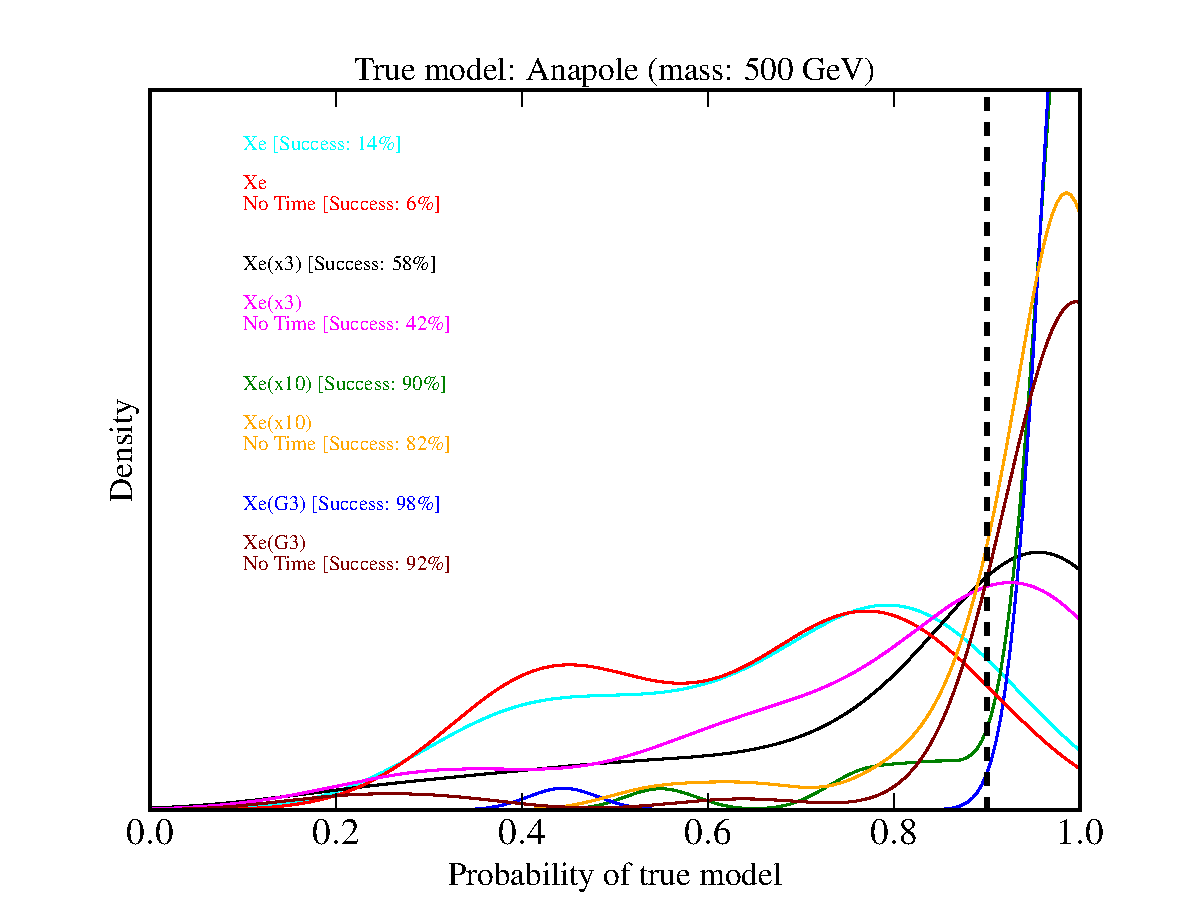
\includegraphics[width=0.5\textwidth]{plots/PDF_500GeV_Anapole_50sims_Xe_Xe3x_Xe10x_XeG3_TNT_noGF.pdf}
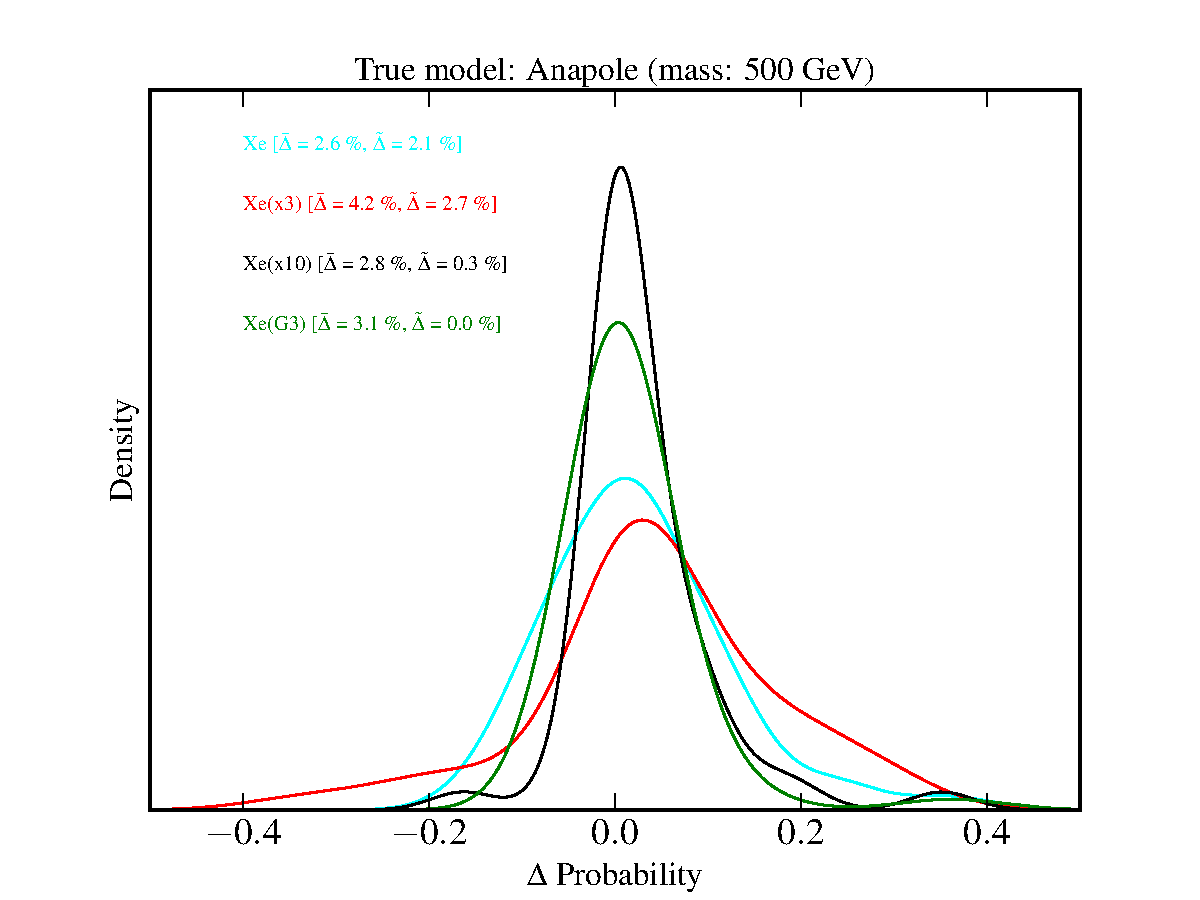
\includegraphics[width=0.5\textwidth]{plots/PDF_500GeV_Anapole_50sims_Xe_Xe3x_Xe10x_XeG3_noGF_TimeDIFF.pdf}
\caption{\label{fig:500gev_anapole_XeFull_tnt_noGF}}
\end{figure*}

\begin{figure*}
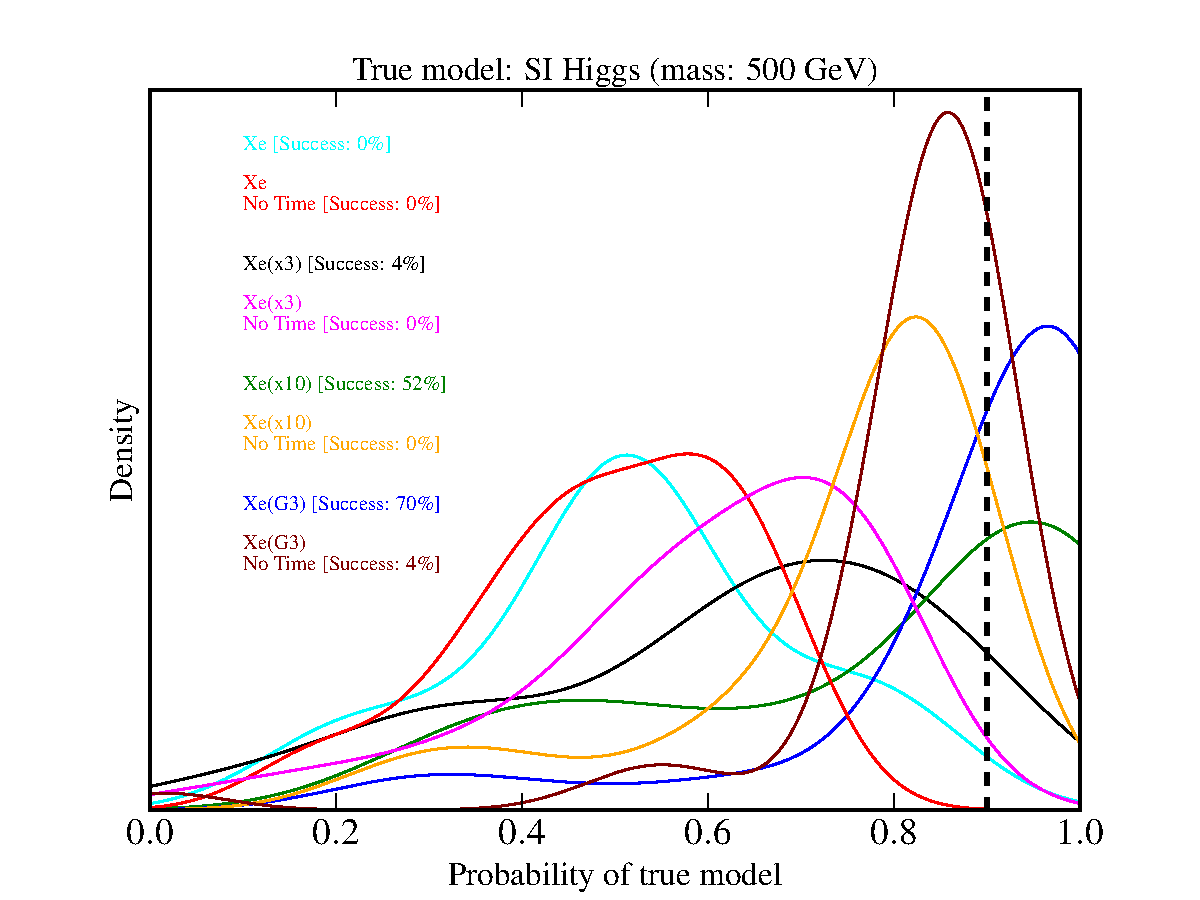
\includegraphics[width=0.5\textwidth]{plots/PDF_500GeV_SI_Higgs_50sims_Xe_Xe3x_Xe10x_XeG3_TNT_noGF.pdf}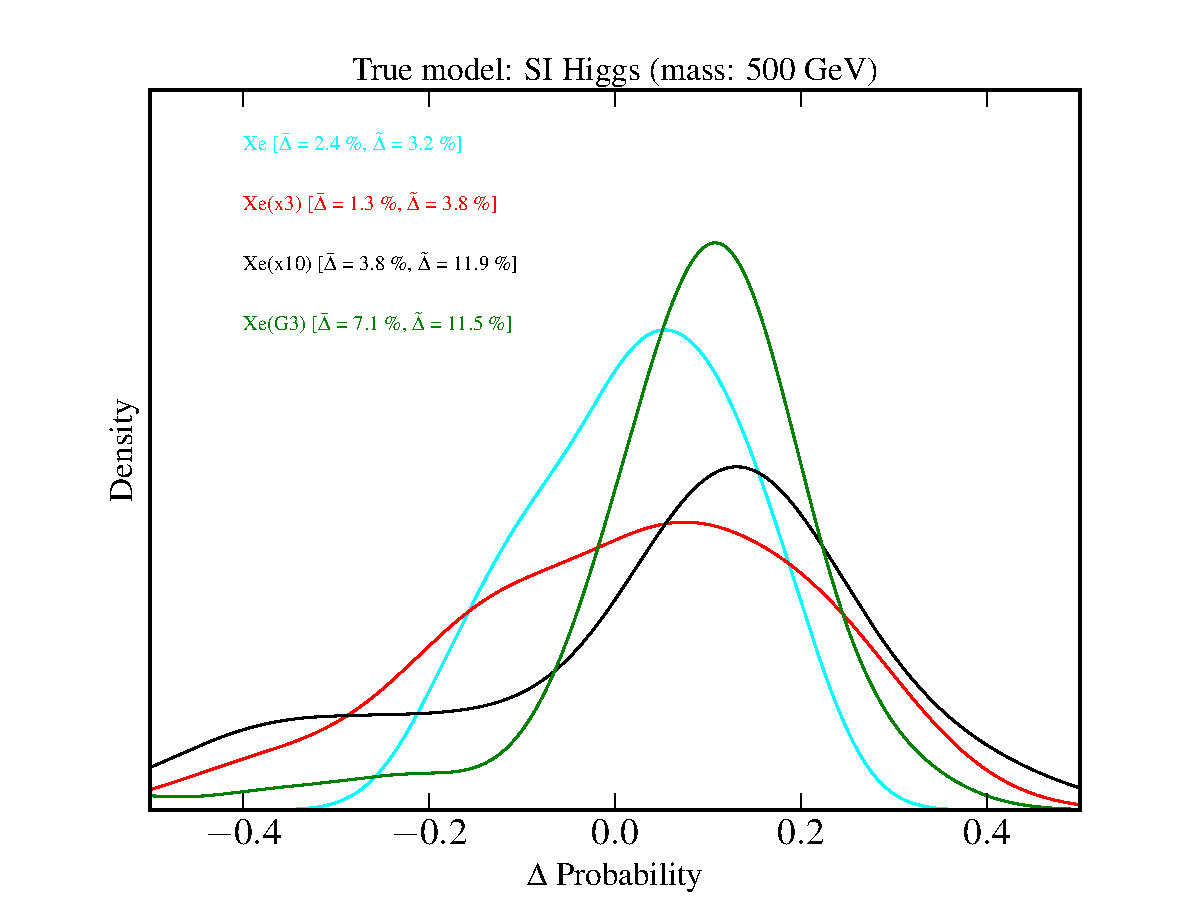
\includegraphics[width=0.5\textwidth]{plots/PDF_500GeV_SI_Higgs_50sims_Xe_Xe3x_Xe10x_XeG3_noGF_TimeDIFF.pdf}
\caption{\label{fig:500gev_si_XeFull_tnt_noGF}}
\end{figure*}




\section{Results}

\section{Conclusions}



\bibliographystyle{JHEP}
\bibliography{mod-sel}

\end{document}